\documentclass[12pt, a4paper]{article}

\usepackage[utf8]{inputenc}
\usepackage[T1]{fontenc}
\usepackage[italian]{babel}
\usepackage{geometry}
\geometry{a4paper, margin=2.5cm}

\usepackage{setspace}
\onehalfspacing

\usepackage{titlesec}
\usepackage{titling}
\usepackage{abstract}
\usepackage{fancyhdr}
\usepackage{graphicx}
\usepackage{float}
\usepackage{amsmath}
\usepackage{amssymb}
\usepackage{listings}
\usepackage{xcolor}
\usepackage{hyperref}
\usepackage{booktabs}
\usepackage{array}
\usepackage{enumitem}
\usepackage{float}
\usepackage{caption}
\usepackage{tikz}
\usepackage[utf8]{inputenc}
\usepackage{pmboxdraw}
\usetikzlibrary{trees, positioning, arrows.meta}

% ============================================================
% STILE LISTATI DI CODICE
% ============================================================
\definecolor{codebg}{rgb}{0.97,0.97,0.97}
\definecolor{codegreen}{rgb}{0.0, 0.5, 0.0}
\definecolor{codepurple}{rgb}{0.5, 0.0, 0.5}
\definecolor{codeblue}{rgb}{0.0, 0.0, 0.7}
\definecolor{codegray}{rgb}{0.4, 0.4, 0.4}

\lstdefinestyle{pythonstyle}{
    backgroundcolor=\color{codebg},
    commentstyle=\color{codegreen}\itshape,
    keywordstyle=\color{codeblue}\bfseries,
    stringstyle=\color{codepurple},
    numberstyle=\tiny\color{codegray},
    basicstyle=\ttfamily\small,
    breakatwhitespace=false,
    breaklines=true,
    captionpos=b,
    keepspaces=true,
    numbers=left,
    numbersep=8pt,
    showspaces=false,
    showstringspaces=false,
    showtabs=false,
    tabsize=4,
    frame=single,
    framerule=0.4pt,
    rulecolor=\color{gray!40},
    xleftmargin=15pt,
    xrightmargin=5pt,
    language=Python
}
\lstset{style=pythonstyle}

% ============================================================
% INTESTAZIONE E PIÈ DI PAGINA
% ============================================================
\pagestyle{fancy}
\fancyhf{}
\rhead{\small Convertitore It-Yo}
\lhead{\small Tecnologie del linguaggio naturale}
\cfoot{\thepage}
\renewcommand{\headrulewidth}{0.4pt}

% ============================================================
% TITOLO
% ============================================================
\title{
    \vspace{-1cm}
    {\large Relazione tecnica per il corso di}\\[0.3cm]
    {\large \textit{Tecnologie del linguaggio naturale}}\\[1cm]
    \rule{\linewidth}{1.5pt}\\[0.5cm]
    {\LARGE \textbf{Convertitore Lessicale Italiano $\rightarrow$ Yoda}}\\[0.3cm]
    {\large algoritmo CKY e trasformazione dell'ordine delle parole}\\[0.3cm]
    \rule{\linewidth}{1.5pt}
}

\author{
    \begin{tabular}[t]{c}
        Franco Andrea \\
        Iudice Samuele \\
        Olivero Alessandro \\[0.4cm]
        \small Università degli Studi di Torino \\
        \small Corso di Laurea Magistrale in Informatica
    \end{tabular}
}
\date{Anno Accademico 2025/2026}

% ============================================================
% DOCUMENTO
% ============================================================
\begin{document}

\maketitle
\thispagestyle{empty}
\vspace{1cm}

% ============================================================
% ABSTRACT
% ============================================================
\begin{abstract}
\noindent
L'obbiettivo del progetto è l'implementazione di un sistema per la conversione automatica di frasi dall'italiano allo Yodish, variante sintattica ispirata al linguaggio di Yoda nella saga di Guerre Stellari. 
Sviluppato in Python, il software integra un parser CKY per l'analisi a costituenti e un modulo di trasformazione ricorsiva degli alberi di derivazione. Questa relazione analizza l'intero workflow, dalla 
modellazione della grammatica alla manipolazione sintattica, discutendo i risultati ottenuti e i limiti dell'approccio rule-based. 
Nel corso della realizzazione progettuale abbiamo adottato il materiale didattico del docente come riferimento per l'apparato teorico e nozionistico, avvalendoci invece del supporto dell'intelligenza artificiale generativa come ausilio operativo nella fase di esecuzione pratica del progetto.
\end{abstract}

\newpage
\tableofcontents
\newpage

% ============================================================
% 1. INTRODUZIONE
% ============================================================
\section{Introduzione}

Il progetto svolto presenta un sistema di conversione sintattica dall'italiano standard (SVX) all'ordine (XSV) tipico dello yodish. Sviluppato in Python, il software modella il linguaggio tramite grammatiche context-free (CFG) in Forma Normale di Chomsky (CNF).

Lo sviluppo progettuale si articola in tre fasi principali:
\begin{itemize}
    \item \textbf{Parsing CKY}: analisi bottom-up della frase tramite un lessico e regole grammaticali definiti in formato JSON.
    \item \textbf{Trasformazione}: manipolazione ricorsiva dell'albero di derivazione per il riposizionamento dei costituenti sintattici.
    \item \textbf{Linearizzazione}: generazione della stringa finale a partire dalle foglie dell'albero trasformato.
\end{itemize}

L'approccio adottato garantisce una netta separazione tra logica algoritmica e base di conoscenza linguistica, consentendo maggiore flessbilità e portabilità del sistema.

% ============================================================
% 2. Applicazioni teoriche
% ============================================================
\section{Applicazioni teoriche}

\subsection{Grammatiche Context-Free}

Una grammatica context-free è una quadrupla $G = (V, \Sigma, R, S)$ dove:
\begin{itemize}
    \item $V$ è un insieme finito di simboli non-terminali.
    \item $\Sigma$ è un insieme finito di terminali.
    \item $R$ è un insieme finito di regole di produzione della forma
          $A \rightarrow \alpha$.
    \item $S \in V$ è il simbolo iniziale detto assioma.
\end{itemize}
Una stringa $w \in \Sigma^*$ è generata da $G$ se esiste una derivazione
$S \Rightarrow^* w$. Il linguaggio $L(G)$ generato dalla grammatica è l'insieme di
tutte le stringhe derivabili dall'assioma.


\subsection{Forma Normale di Chomsky}

Un algoritmo di parsing efficiente come CKY richiede che la grammatica sia in
\textbf{Forma Normale di Chomsky} (CNF). Una CFG è in CNF se tutte le regole
di produzione sono della forma:
\[
    A \rightarrow BC \quad \text{oppure} \quad A \rightarrow a
\]
dove $A, B, C \in V$ e $a \in \Sigma$, ovvero, ogni regola produce
esattamente due non-terminali oppure un singolo terminale.

\subsection{L'Algoritmo CKY}

L'algoritmo \textbf{CKY} (da Cocke, Kasami e Younger) è un algoritmo
di parsing bottom-up per grammatiche in CNF, basato su programmazione dinamica.
Dato l'input $w = w_1 w_2 \cdots w_n$, l'algoritmo costruisce una
tabella triangolare $T$ di dimensione $n \times n$, dove la cella
$T[i][j]$ contiene l'insieme dei non-terminali che possono derivare la sottostringa
$w_i w_{i+1} \cdots w_j$.

\paragraph{Algoritmo:}
\begin{enumerate}
    \item \textbf{Inizializzazione}: per ogni $i$ da 1 a $n$, inserire in $T[i][i]$
          tutti i non-terminali $A$ tali che $A \rightarrow w_i$ è una regola lessicale.
    \item \textbf{Riempimento}: per ogni lunghezza di span $\ell$ da 2 a $n$, per ogni
          inizio $i$ e fine $j = i + \ell - 1$, per ogni punto di taglio $k$ da $i$ a
          $j-1$: se $B \in T[i][k]$ e $C \in T[k+1][j]$ e $A \rightarrow BC \in R$,
          allora inserire $A$ in $T[i][j]$.
    \item \textbf{Accettazione}: la frase è riconosciuta se e solo se $S \in T[1][n]$.
\end{enumerate}
L'efficienza dell'algoritmo deriva dalla tecnica della programmazione "dinamica", che evita di ricalcolare più volte gli stessi sotto-alberi sintattici,
risolvendo il problema del parsing in tempo polinomiale invece che esponenziale.

% ============================================================
% 3. STRUTTURA DEL PROGETTO
% ============================================================
\section{Struttura Progettuale}

Il progetto è organizzato in tre componenti principali:

\begin{table}[H]
\centering
\begin{tabular}{>{\ttfamily}l l p{7cm}}
\toprule
\normalfont{File} & Tipo & Descrizione \\
\midrule
\texttt{convertitore\_yoda.py}& Codice Python & Modulo principale: parsing, trasformazione, CLI \\
Lexicon.json & Dati JSON & Lessico italiano con etichette POS \\
regole\_binarie.json & Dati JSON & Regole binarie della grammatica in CNF \\
\bottomrule
\end{tabular}
\end{table}

\subsection{Lexicon (\texttt{Lexicon.json})}

Lexicon è un dizionario in file JSON che mappa ogni parola italiana a una lista di
categorie grammaticali (POS tag). Ad esempio:
\begin{figure}[H] % [H] forza l'immagine esattamente in questo punto
    \centering % Centra l'immagine
    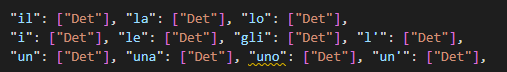
\includegraphics[width=0.8\textwidth]{lexicon} % Non serve l'estensione (.png, .jpg)
    \caption{Organizzazione dei dati nel file Lexicon.JSON}
\end{figure}

\subsection{Le Regole Grammaticali (\texttt{regole\_binarie.json})}

Il file contiene le regole binarie della grammatica in CNF, dove la chiave è la
coppia di figli e il valore è la lista dei possibili genitori. La scelta di
invertire la direzione rispetto alla notazione tradizionale (dai figli
al genitore) è una ottimizzazione utile all'algoritmo CKY: durante il parsing si cerca
quali genitori sono compatibili con una coppia di figli già riconosciuti, non
il contrario.

\begin{figure}[H] % [H] forza l'immagine esattamente in questo punto
    \centering % Centra l'immagine
    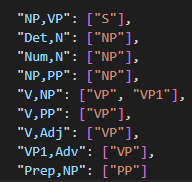
\includegraphics[width=0.3\textwidth]{regole} % Non serve l'estensione (.png, .jpg)
    \caption{Organizzazione delle regole binarie nel file JSON}
    
\end{figure}

La funzione \texttt{carica\_dizionari()} in fase di inizializzazione converte le
chiavi stringa (es. \texttt{"Det,N"}) nelle tuple Python richieste dall'algoritmo
(es. \texttt{('Det', 'N')}).

% ============================================================
% 4. IMPLEMENTAZIONE
% ============================================================
\section{Implementazione}

\subsection{La Classe Nodo}

L'albero di derivazione è rappresentato tramite la classe Nodo, che
implementa un nodo di albero n-ario con tre attributi:

\begin{itemize}
    \item \texttt{label}: il simbolo grammaticale del nodo (es. \texttt{'NP'},
          \texttt{'VP'}) oppure la parola stessa nelle foglie.
    \item \texttt{children}: lista di nodi figli.
    \item \texttt{word}: la parola (solo per le foglie lessicali).
\end{itemize}

I nodi foglia sono distinti da quelli interni tramite il metodo
\texttt{is\_leaf()}, che verifica se la lista \texttt{children} è vuota.

La struttura è volutamente semplice per facilitare la visita ricorsiva sia nella
stampa (\texttt{pretty\_print}) che nella trasformazione Yoda.

\begin{figure}[H] % [H] forza l'immagine esattamente in questo punto
    \centering % Centra l'immagine
    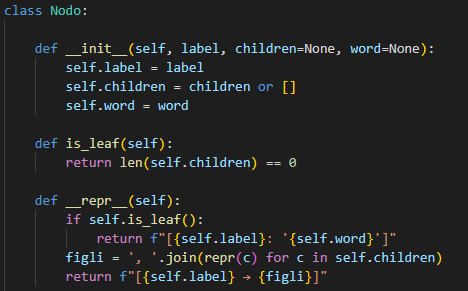
\includegraphics[width=0.6\textwidth]{classenodo} % Non serve l'estensione (.png, .jpg)
    \caption{Implementazione dell'albero di derivazione}  
\end{figure}

Il metodo \texttt{pretty\_print()} produce una rappresentazione visuale ad albero
nel terminale, con connettori grafici ASCII (\texttt{├──}, \texttt{└──}, \texttt{│})
per dare in output un risultato più chiaro all'utente.

\subsection{L'Algoritmo CKY: Implementazione}

La funzione \texttt{cky\_parse(sentence)} riceve una lista di parole tokenizzate
e restituisce il nodo radice dell'albero di derivazione (etichettato \texttt{'S'})
oppure \texttt{None} se la frase non è riconosciuta dalla grammatica.

L'implementazione usa una tabella tridimensionale \texttt{table[i][j]} dove ogni
cella è un dizionario \texttt{\{simbolo: Nodo\}}. Questa scelta — memorizzare
direttamente il nodo invece del semplice booleano — consente di ricostruire
l'albero durante il parsing senza una fase separata di \textit{backtracking}.

\begin{figure}[H] % [H] forza l'immagine esattamente in questo punto
    \centering % Centra l'immagine
    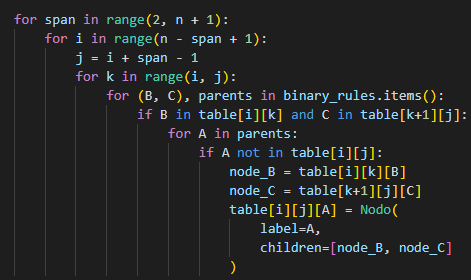
\includegraphics[width=0.6\textwidth]{cky} % Non serve l'estensione (.png, .jpg)
    \caption{Implementazione dell'algoritmo cky}
\end{figure}


L'algoritmo gestisce l'ambiguità grammaticale in modo deterministico restituendo unicamente il primo albero derivato, 
la cui struttura dipende esclusivamente dall'ordine di iterazione delle regole nel dizionario.

\subsection{Trasformazione in Ordine Yoda}

La funzione \texttt{trasforma\_in\_yoda()},
che visita l'albero in post-ordine (prima i figli, poi il nodo corrente) e
riorganizza i sottoalberi laddove trova la struttura sintattica canonica italiana.

La regola principale è: ogni nodo \texttt{S} con struttura $S \rightarrow NP\ VP$
viene trasformato in $S\_yoda \rightarrow Comp\ NP\ V$, dove \texttt{Comp} è il
complemento contenuto nel VP. In altre parole, il complemento viene spostato in
posizione iniziale di frase.

Sono gestiti tre casi distinti:

\paragraph{Caso 1: Frase transitiva semplice} $VP \rightarrow V\ X$ con $X \in \{NP, PP, Adj\}$
\[
    S \rightarrow NP\ (VP \rightarrow V\ Comp)
    \quad \Longrightarrow \quad
    S\_yoda \rightarrow Comp\ NP\ V
\]

\paragraph{Caso 2: Frase con avverbio} $VP \rightarrow VP1\ Adv$ con $VP1 \rightarrow V\ NP$
\[
    S \rightarrow NP\ (VP \rightarrow (VP1 \rightarrow V\ NP)\ Adv)
    \quad \Longrightarrow \quad
    S\_yoda \rightarrow NP\ Sogg\ V\ Adv
\]

\paragraph{Caso 3: Frase intransitiva} $VP \rightarrow V$ (solo verbo)
\[
    S \rightarrow NP\ (VP \rightarrow V)
    \quad \Longrightarrow \quad
    S\_yoda \rightarrow NP\ V
\]
(nessuna trasposizione, l'ordine resta invariato poiché non c'è complemento da anteporre)  Trasformazione Caso 1 -- VP con complemento diretto

\begin{figure}[H] % [H] forza l'immagine esattamente in questo punto
    \centering % Centra l'immagine
    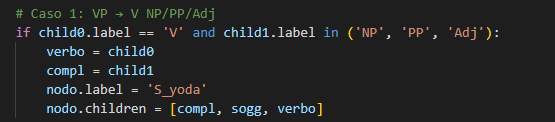
\includegraphics[width=0.8\textwidth]{caso1nodo} % Non serve l'estensione (.png, .jpg)
    \caption{Trasformazione Caso 1 -- VP con complemento diretto}
\end{figure}

\subsection{Linearizzazione e Post-processing}

La funzione \texttt{raccogli\_foglie()} effettua una visita DFS (depth-first,
in-order) sull'albero trasformato, raccogliendo le parole nelle foglie da sinistra
a destra. La funzione \texttt{converti\_in\_yoda()} applica infine un post-processing
minimo:

\begin{itemize}
    \item Le parole vengono rese minuscole, salvo i \textit{nomi propri}, che
          vengono identificati come parole che appaiono nel lessico con entrambi
          i tag \texttt{N} e \texttt{NP} e iniziano con la maiuscola.
    \item La prima parola della frase Yoda viene capitalizzata.
\end{itemize}


% ============================================================
% ESEMPIO DI ESECUZIONE
% ============================================================
\section{Esempio di Esecuzione}

Per illustrare concretamente il funzionamento del sistema, si considera la frase
di input \textit{``Tu hai amici lì''}.

\subsection{Albero di Derivazione Originale}

La frase viene tokenizzata in \texttt{[Tu, hai, amici, lì]}. Il parser CKY
riconosce la struttura seguente:

\begin{figure}[H]
\centering
\begin{tikzpicture}[
    every node/.style={font=\small\ttfamily},
    level 1/.style={sibling distance=5cm, level distance=1.3cm},
    level 2/.style={sibling distance=2.5cm, level distance=1.3cm},
    level 3/.style={sibling distance=1.3cm, level distance=1.2cm},
    edge from parent/.style={draw, -}
]
\node {S}
    child { node {NP}
        child { node {Tu} }
    }
    child { node {VP}
        child { node {VP1}
            child { node {V}
                child { node {hai} }
            }
            child { node {NP}
                child { node {amici} }
            }
        }
        child { node {Adv}
            child { node {lì} }
        }
    };
\end{tikzpicture}
\caption{Albero di derivazione della frase ``Tu hai amici lì''}
\end{figure}

\subsection{Albero Trasformato in Ordine Yoda}

La funzione \texttt{trasforma\_in\_yoda()} identifica la struttura
\\$S \rightarrow NP\ (VP \rightarrow (VP1 \rightarrow V\ NP)\ Adv)$
(Caso 2) e riorganizza le costituenti nell'ordine $Comp\ Sogg\ V\ Adv$:

\begin{figure}[H]
\centering
\begin{tikzpicture}[
    every node/.style={font=\small\ttfamily},
    level 1/.style={sibling distance=3.5cm, level distance=1.3cm},
    level 2/.style={sibling distance=1.5cm, level distance=1.2cm},
    edge from parent/.style={draw, -}
]
\node {S\_yoda}
    child { node {NP}
        child { node {amici} }
    }
    child { node {NP}
        child { node {Tu} }
    }
    child { node {V}
        child { node {hai} }
    }
    child { node {Adv}
        child { node {lì} }
    };
\end{tikzpicture}
\caption{Albero trasformato in ordine Yoda: ``Amici tu hai lì''}
\end{figure}

La linearizzazione delle foglie produce la frase finale:
\begin{center}
    \textbf{Input ITALIANO:} \textit{Tu hai amici lì} \\[0.3cm]
    \textbf{Output YODISH:} \textit{Amici tu hai lì}
\end{center}

% ============================================================
% 7. LIMITI E POSSIBILI ESTENSIONI
% ============================================================

\section{Test e Limiti del Sistema}

In questa sezione vengono analizzate le prestazioni del convertitore attraverso casi di test reali, verificando sia la corretta capacità di trasformazione sintattica sia le restrizioni strutturali del parser CKY implementato.

\subsection{Casi di Test (Successo)}
Le frasi riportate di seguito sono state elaborate correttamente, poiché i lemmi appartengono al \texttt{Lexicon.json} e le strutture rispettano le regole in Forma Normale di Chomsky (CNF) definite nel progetto.

\begin{table}[h!]
\centering
\small
\begin{tabular}{|l|l|l|p{5cm}|}
\hline
\textbf{Tipologia} & \textbf{Input Italiano} & \textbf{Output Yodish} & \textbf{Analisi} \\ \hline
Semplice & \textit{Luke usa la forza} & La forza Luke usa & Il complemento oggetto "la forza" viene correttamente anteposto al soggetto. \\ \hline
Con Numerale & \textit{Vader distrugge due droni} & Due droni Vader distrugge & Il sintagma nominale (NP) composto da numerale e nome viene spostato integralmente. \\ \hline
Con Avverbio & \textit{Io vedo sith qui} & Sith io vedo qui & L'avverbio "qui" mantiene la posizione finale secondo la logica del Caso 2. \\ \hline
Sogg. Pronome & \textit{Lui mangia la mela} & La mela lui mangia & Corretto riconoscimento dei pronomi personali come sintagmi nominali. \\ \hline
\end{tabular}
\caption{Esempi di trasformazioni eseguite con successo dal sistema.}
\label{tab:test_successo}
\end{table}

\subsection{Limiti del Sistema}
Attraverso una fase di "stress test" con parole estratte esclusivamente dal lessico fornito, sono emersi i limiti intrinseci dell'approccio rule-based del sistema:

\begin{itemize}
    \item \textbf{Posizionamento degli Aggettivi:} Sebbene termini come \textit{"oscuro"} o \textit{"potente"} siano presenti nel lessico come \texttt{Adj}, la grammatica attuale fallisce il parsing di frasi come \textit{"Il lato oscuro vince"}. Ciò è dovuto alla mancanza di una regola binaria che gestisca la sequenza \texttt{N, Adj} all'interno di un NP.
    \item \textbf{Ambiguità Lessicale:} Parole come \textit{"rosso"} o \textit{"nero"} sono caricate con doppio tag (\texttt{Adj} e \texttt{N}). Il parser restituisce solo il primo albero derivato trovato, ignorando potenziali interpretazioni alternative che potrebbero influenzare la qualità della traduzione.
    \item \textbf{Mancanza di Flessione (Lemmatizzazione):} Il sistema fallisce se viene inserita una forma verbale non esplicitamente mappata. Ad esempio, mentre \textit{"Noi abbiamo speranza"} viene riconosciuto, \textit{"Noi avevamo speranza"} produce un errore poiché "avevamo" non figura nel \texttt{Lexicon.json}.
    \item \textbf{Strutture Complesse:} Il sistema non è in grado di processare complementi introdotti da preposizioni articolate (es. \textit{"della"}, \textit{"nella"}) a meno che non vengano inserite manualmente come token singoli, limitando di fatto il linguaggio naturale arbitrario.
\end{itemize}

\subsection{Conclusioni sui Test}
I test confermano che il cuore algoritmico (CKY e trasformazione ricorsiva) è solido e performante per l'uso didattico previsto. Tuttavia, la "Yodificazione" è attualmente limitata alla struttura della frase principale: il sistema è ottimizzato per spostare complementi diretti, ma richiede un arricchimento delle regole binarie per gestire correttamente subordinate o strutture aggettivali complesse.


% ============================================================
% 9. CONCLUSIONI
% ============================================================
\section{Conclusioni e sviluppi futuri}

Il progetto IT-YO ha consentito di mettere in pratica i concetti fondamentali
di analisi sintattica formale appresi durante le lezioni frontali.
Il sistema è funzionante per un sottoinsieme controllato di frasi italiane e
produce output corretti sui casi di test previsti. La separazione tra grammatica
e logica di parsing rende il sistema facilmente
estendibile per coprire nuove costruzioni sintattiche è sufficiente aggiungere
voci al lessico e regole al file JSON, senza modificare l'algoritmo.
Dal punto di vista didattico, il progetto illustra concretamente come la teoria
delle grammatiche formali si traduca in un sistema computazionale funzionante,
e come la manipolazione degli alberi di derivazione sia uno strumento potente
per operare trasformazioni linguistiche strutturate.
Tra i possibili sviluppi futuri, l'integrazione con un PoS tagger automatico e
l'estensione della grammatica a costruzioni più complesse rappresentano le
direzioni più promettenti per avvicinare il sistema a un uso su frasi naturali
non vincolate.

\end{document}